\section{迁移率与温度和杂质浓度的关系}
在\xref{sec:载流子的散射}中,我们讨论了各散射机构的散射概率$P$,那么,散射概率$P$是如何与\xref{sec:载流子的漂移运动}中的迁移率$\mu$联系在一起的呢?这是本节要讨论的问题,为此,先要引出平均自由时间的概念。

\subsection{平均自由时间和散射概率的关系}
\begin{BoxFormula}[平均自由时间和散射概率]
    平均自由时间$\tau$是散射概率的倒数
    \begin{Equation}
        \tau=\frac{1}{P}
    \end{Equation}
\end{BoxFormula}
\begin{Proof}
    设$N$个载流子以速度$v$沿某方向运动,用$N(t)$表示在$t$时刻尚未遭到散射的载流子,根据散射概率的定义,在$t$至$(t+\delt{t})$间被散射的载流子数为(即$N(t)$和$N(t+\delt{t})$的差)
    \begin{Equation}
        N(t)-N(t+\delt{t})=N(t)P\delt{t}
    \end{Equation}
    当$\delt{t}$很小,同除$\delt{t}$后取极限
    \begin{Equation}
        \Lim[\delt{t}\to 0]\frac{N(t+\delt{t})-N(t)}{\delt{t}}=-PN(t)
    \end{Equation}
    依据导数的定义
    \begin{Equation}
        \dv{N(t)}{t}=-PN(t)
    \end{Equation}
    这样我们就得到了一个关于$N(t)$的微分方程,其解为
    \begin{Equation}
        N(t)=N_0\e^{-Pt}
    \end{Equation}\nopagebreak
    其中$N_0$即在$t=0$时未被散射的载流子数,随时间演进,未被散射的载流子数以负指数减小。\goodbreak

    在$t$至$t+\dd{t}$间被散射的载流子为$N_0\e^{-P t}\dd{t}$,这些载流子在$t$时才被散射,因此具有的自由时间均为$t$,故$tN_0\e^{-P t}\dd{t}$是这些电子自由时间的总和,将其对时间积分,并除以$N_0$
    \begin{Equation}
        \tau=\frac{1}{N_0}\Int[0][\infty]tN(t)\dd{t}=\frac{1}{N_0}\Int[0][\infty]tN_0\e^{-P t}\dd{t}
    \end{Equation}
    这样得到的就是平均自由时间,积分的结果
    \begin{Equation}*
        \tau=\frac{1}{P}\qedhere
    \end{Equation}
\end{Proof}

\subsection{平均自由时间和迁移率的关系}

\begin{BoxFormula}[平均自由时间和迁移率的关系]
    平均自由时间$\tau$和迁移率的关系是
    \begin{Equation}&[]
        \mu_\text{n}=\frac{q\tau_\text{n}}{\mne}\qquad
        \mu_\text{p}=\frac{q\tau_\text{p}}{\mpe}
    \end{Equation}
\end{BoxFormula}
\begin{Proof}
    设载流子的有效质量为$m^{*}$,不妨记外加电场$\Emf$的方向为$x$方向,假若在$t=0$时载流子恰好遭到散射,散射后沿$x$方向的速度是$v_{x0}$,经过时间$t$后又遭到散射,在散射前的速度为
    \begin{Equation}&[1]
        v_x=v_{x0}\pm\frac{q}{m^{*}}\Emf t
    \end{Equation}
    这里正负号分别对应载流子为空穴和电子的情形。

    由于每次散射后的速度是随机的,因此\xrefpeq{1}中,第一项$v_{x0}$的均值$\bar{v_{x0}}$应当为零,第二项均值的计算关键在于“经过时间$t$发生碰撞”,其平均值即平均自由时间$\tau$,因而
    \begin{Equation}
        \bar{v_x}=\pm\frac{q}{m^{*}}\Emf \tau
    \end{Equation}
    根据\fancyref{def:迁移率}
    \begin{Equation}
        \mu=\frac{\abs{\bar{v_x}}}{\Emf}=\frac{q\tau}{m^{*}}
    \end{Equation}
    在上式中,就$m^{*},\tau$分别代入$\mne,\mpe$和$\tau_\text{n},\tau{p}$,即得\xrefpeq{}。
\end{Proof}
这里我们可以总结出了“电导率--迁移率--平均自由时间--散射概率”的关系
\begin{Gather}[10pt]
    \sigma_n\xleq[$nq$][\xref{fml:半导体的迁移率与电导率}]\mu_\text{n}\xleq[$q/\mne$][\xref{fml:平均自由时间和迁移率的关系}]\tau_\text{n}\xleq[][\xref{fml:平均自由时间和散射概率}] P_\text{n}^{-1}\\
    \sigma_p\xleq[$pq$][\xref{fml:半导体的迁移率与电导率}]\mu_\text{p}\xleq[$q/\mpe$][\xref{fml:平均自由时间和迁移率的关系}]\tau_\text{p}\xleq[][\xref{fml:平均自由时间和散射概率}] P_\text{p}^{-1}
\end{Gather}

\subsection{迁移率与杂质和温度的关系}
由于$\mu\propto P^{-1}$,因此,对于不同的散射机构,很容易得到迁移率与温度的关系。\setpeq{迁移率与杂质和温度的关系}

根据\fancyref{fml:电离杂质的散射概率}
\begin{Equation}&[1]
    \mu_\text{i}\propto N_\text{i}T^{3/2}
\end{Equation}

根据\fancyref{fml:声学波的散射概率}
\begin{Equation}&[2]
    \mu_\text{s}\propto T^{-3/2}
\end{Equation}

根据\fancyref{fml:光学波的散射概率}
\begin{Equation}&[3]
    \mu_\text{o}\propto\exp(\hbar\omega_\text{l}/\kB T)-1
\end{Equation}
但需要注意的是,对于若干散射机构同时作用的情形,散射概率是可以相加的,迁移率则不能相加,相反,应适用的是,总的迁移率的倒数,是各个散射机构迁移率的倒数和。

例如,对于硅和锗,它们的迁移率应当为
\begin{Equation}
    \frac{1}{\mu}=\frac{1}{\mu_\text{s}}+\frac{1}{\mu_\text{i}}
\end{Equation}
例如,对于砷化镓这样的半导体,光学波的散射也需要被考虑
\begin{Equation}
    \frac{1}{\mu}=\frac{1}{\mu_\text{s}}+\frac{1}{\mu_\text{i}}+\frac{1}{\mu_\text{o}}
\end{Equation}
我们特别感兴趣的还是硅和锗,由于$\mu_\text{s},\mu_\text{i}$可以写作
\begin{Equation}
    \mu_\text{s}=\frac{q}{m^{*}}\frac{T^{-3/2}}{A}\qquad
    \mu_\text{i}=\frac{q}{m^{*}}\frac{T^{3/2}}{BN_\text{i}}
\end{Equation}
因此,总的迁移率就是
\begin{Equation}
    \mu=\qty[\frac{1}{\mu_\text{s}}+\frac{1}{\mu_\text{i}}]^{-1}=\qty[\frac{m^{*}}{q}\qty(AT^{3/2}+BN_iT^{-3/2})]^{-1}
\end{Equation}
即
\begin{Equation}&[A]
    \mu=\frac{q}{m^{*}}\frac{1}{AT^{3/2}+BN_iT^{-3/2}}
\end{Equation}
这就是硅和锗的迁移率$\mu$与温度$T$和掺杂浓度$N_\text{i}$的关系,在\xref{fig:迁移率的曲线图}中分别进行了绘制\footnote{这里并没有$A,B$的参考值,绘图时$A,B$取值是对照书中的图像大致取的,故只能算作半定量的图像。}。\goodbreak
\begin{Figure}[迁移率的曲线图]
    \begin{FigureSub}[迁移率和温度的关系]
        \hspace{0.25cm}
        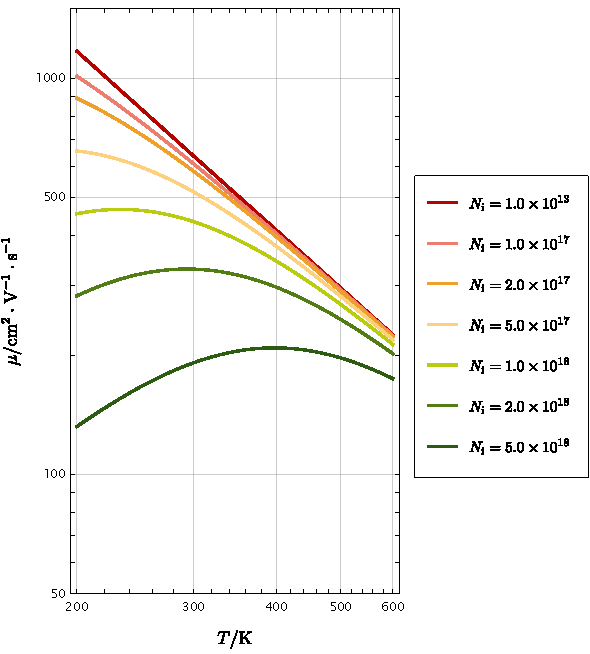
\includegraphics[scale=0.65]
        {Mathematica/output/MobilityT.pdf}
    \end{FigureSub}
    \hspace{1cm}
    \begin{FigureSub}[迁移率和掺杂浓度的关系]
        \hspace{0.25cm}
        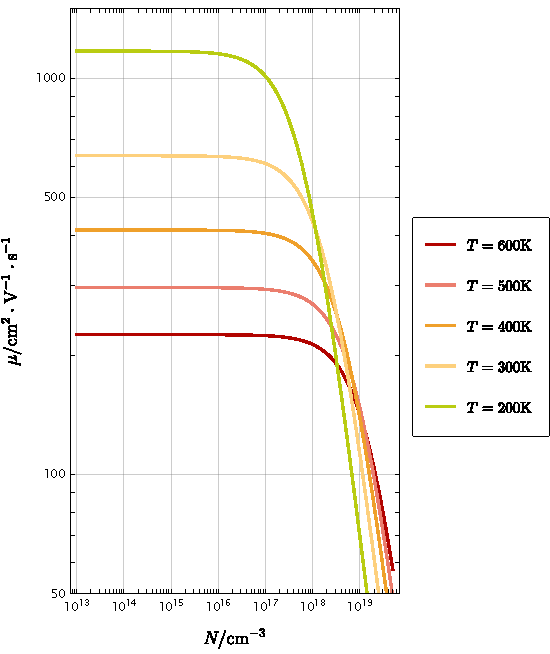
\includegraphics[scale=0.65]
        {Mathematica/output/MobilityN.pdf}
    \end{FigureSub}
\end{Figure}
现在我们来具体讨论迁移率与温度和掺杂浓度的关系
\begin{itemize}
    \item 在\xref{fig:迁移率和温度的关系}中我们看到,对于掺杂浓度较低的样品($N_\text{i}\leq 10^{17}\si{cm^{-3}}$),迁移率随温度迅速减小,在双对数图上表现为斜率为$-3/2$的直线,这是因为$N_i$较小时,\xrefpeq{A}中电离杂质散射项$BN_\text{i}T^{-3/2}$可以忽略的缘故,此时只有声学波散射项$AT^{3/2}$在起作用。而随着掺杂浓度的提高,电离杂质散射的影响在逐渐增强,迁移率随温度减小的趋势趋缓。对于掺杂浓度较高的样品($N_\text{i}\geq 10^{18}\si{cm^{-3}}$),在低温范围,迁移率还会随温度升高缓慢的上升,在温度较高后,迁移率才会逐渐下降,这表明低温时电离杂质散射起主要作用。
    \item 在\xref{fig:迁移率和掺杂浓度的关系}中我们看到,迁移率随掺杂浓度单调递减,掺杂浓度较低时迁移率可以视为定值,掺杂浓度超过$10^{18}\si{cm^{-3}}$后,迁移率将迅速下降,原先迁移率越高的下降的越快。
\end{itemize}
这里我们可能会有困惑,直观上想,温度越高载流子应该越活越,掺杂浓度越高载流子的数量也会更多,好像迁移率反而应该更大?这种错误认知源于对迁移率的概念的不清楚,迁移率代表的是单位电场强度下载流子的漂移速度,而漂移速度能达到多少,关键取决于平均自由时间的长短,温度越高,电子与晶格的碰撞越频繁,掺杂越多,电子与杂质离子相互作用的机会就越多,因此,\empx{更高的温度和更高的掺杂浓度都会缩短平均自由时间,从而导致迁移率下降}。\footnote{换一个角度,或许掺杂导致的迁移率下降可以视为掺杂带来的载流子浓度提升的副作用?}

但事实是,迁移率与掺杂浓度间的关系要远比\xref{fig:迁移率和掺杂浓度的关系}所示的要复杂的多,因为先前的所有分析都是在轻掺杂的背景下考虑的,没有考虑重掺杂的情形。随着半导体器件的不断发展,重掺杂区中载流子的迁移率研究得到重视,\xref{fig:硅的迁移率和掺杂浓度的关系}给出了硅在室温下迁移率和掺杂浓度的关系
\begin{enumerate}
    \item 随着掺杂浓度的增加,迁移率是由一个定值趋于另一个定值,并不会迅速下降。
    \item 在掺杂浓度较低时,电子迁移率趋于$\mu_\text{n}=1330\si{cm^2.V^{-1}.s^{-1}}$
    \item 在掺杂浓度较低时,空穴迁移率趋于$\mu_\text{p}=495\si{cm.V^{-1}.s^{-1}}$
    \item 在掺杂浓度较高时,\empx{载流子作为多子和少子时的迁移率将会出现分歧},这是重掺杂最主要的结论,并且,在一定杂质浓度下,载流子作为少子的迁移率多于作为多子的迁移率。
\end{enumerate}

杂质浓度进入重掺杂区后,少子迁移率大于多子迁移率的原因可以这样理解:重掺杂时杂质能级往往会扩展为杂质能带,因此,多子在运动过程中,会时不时的被杂质能带俘获,这样被俘获、再释放、再俘获的过程,使得平均自由时间减小,进而,使得多子的迁移率减小。相反的,重掺杂时,少子的运动仍然是在正常的能带中进行的,因此没有受到上述效应的影响。

\begin{Figure}[硅的迁移率和掺杂浓度的关系]
    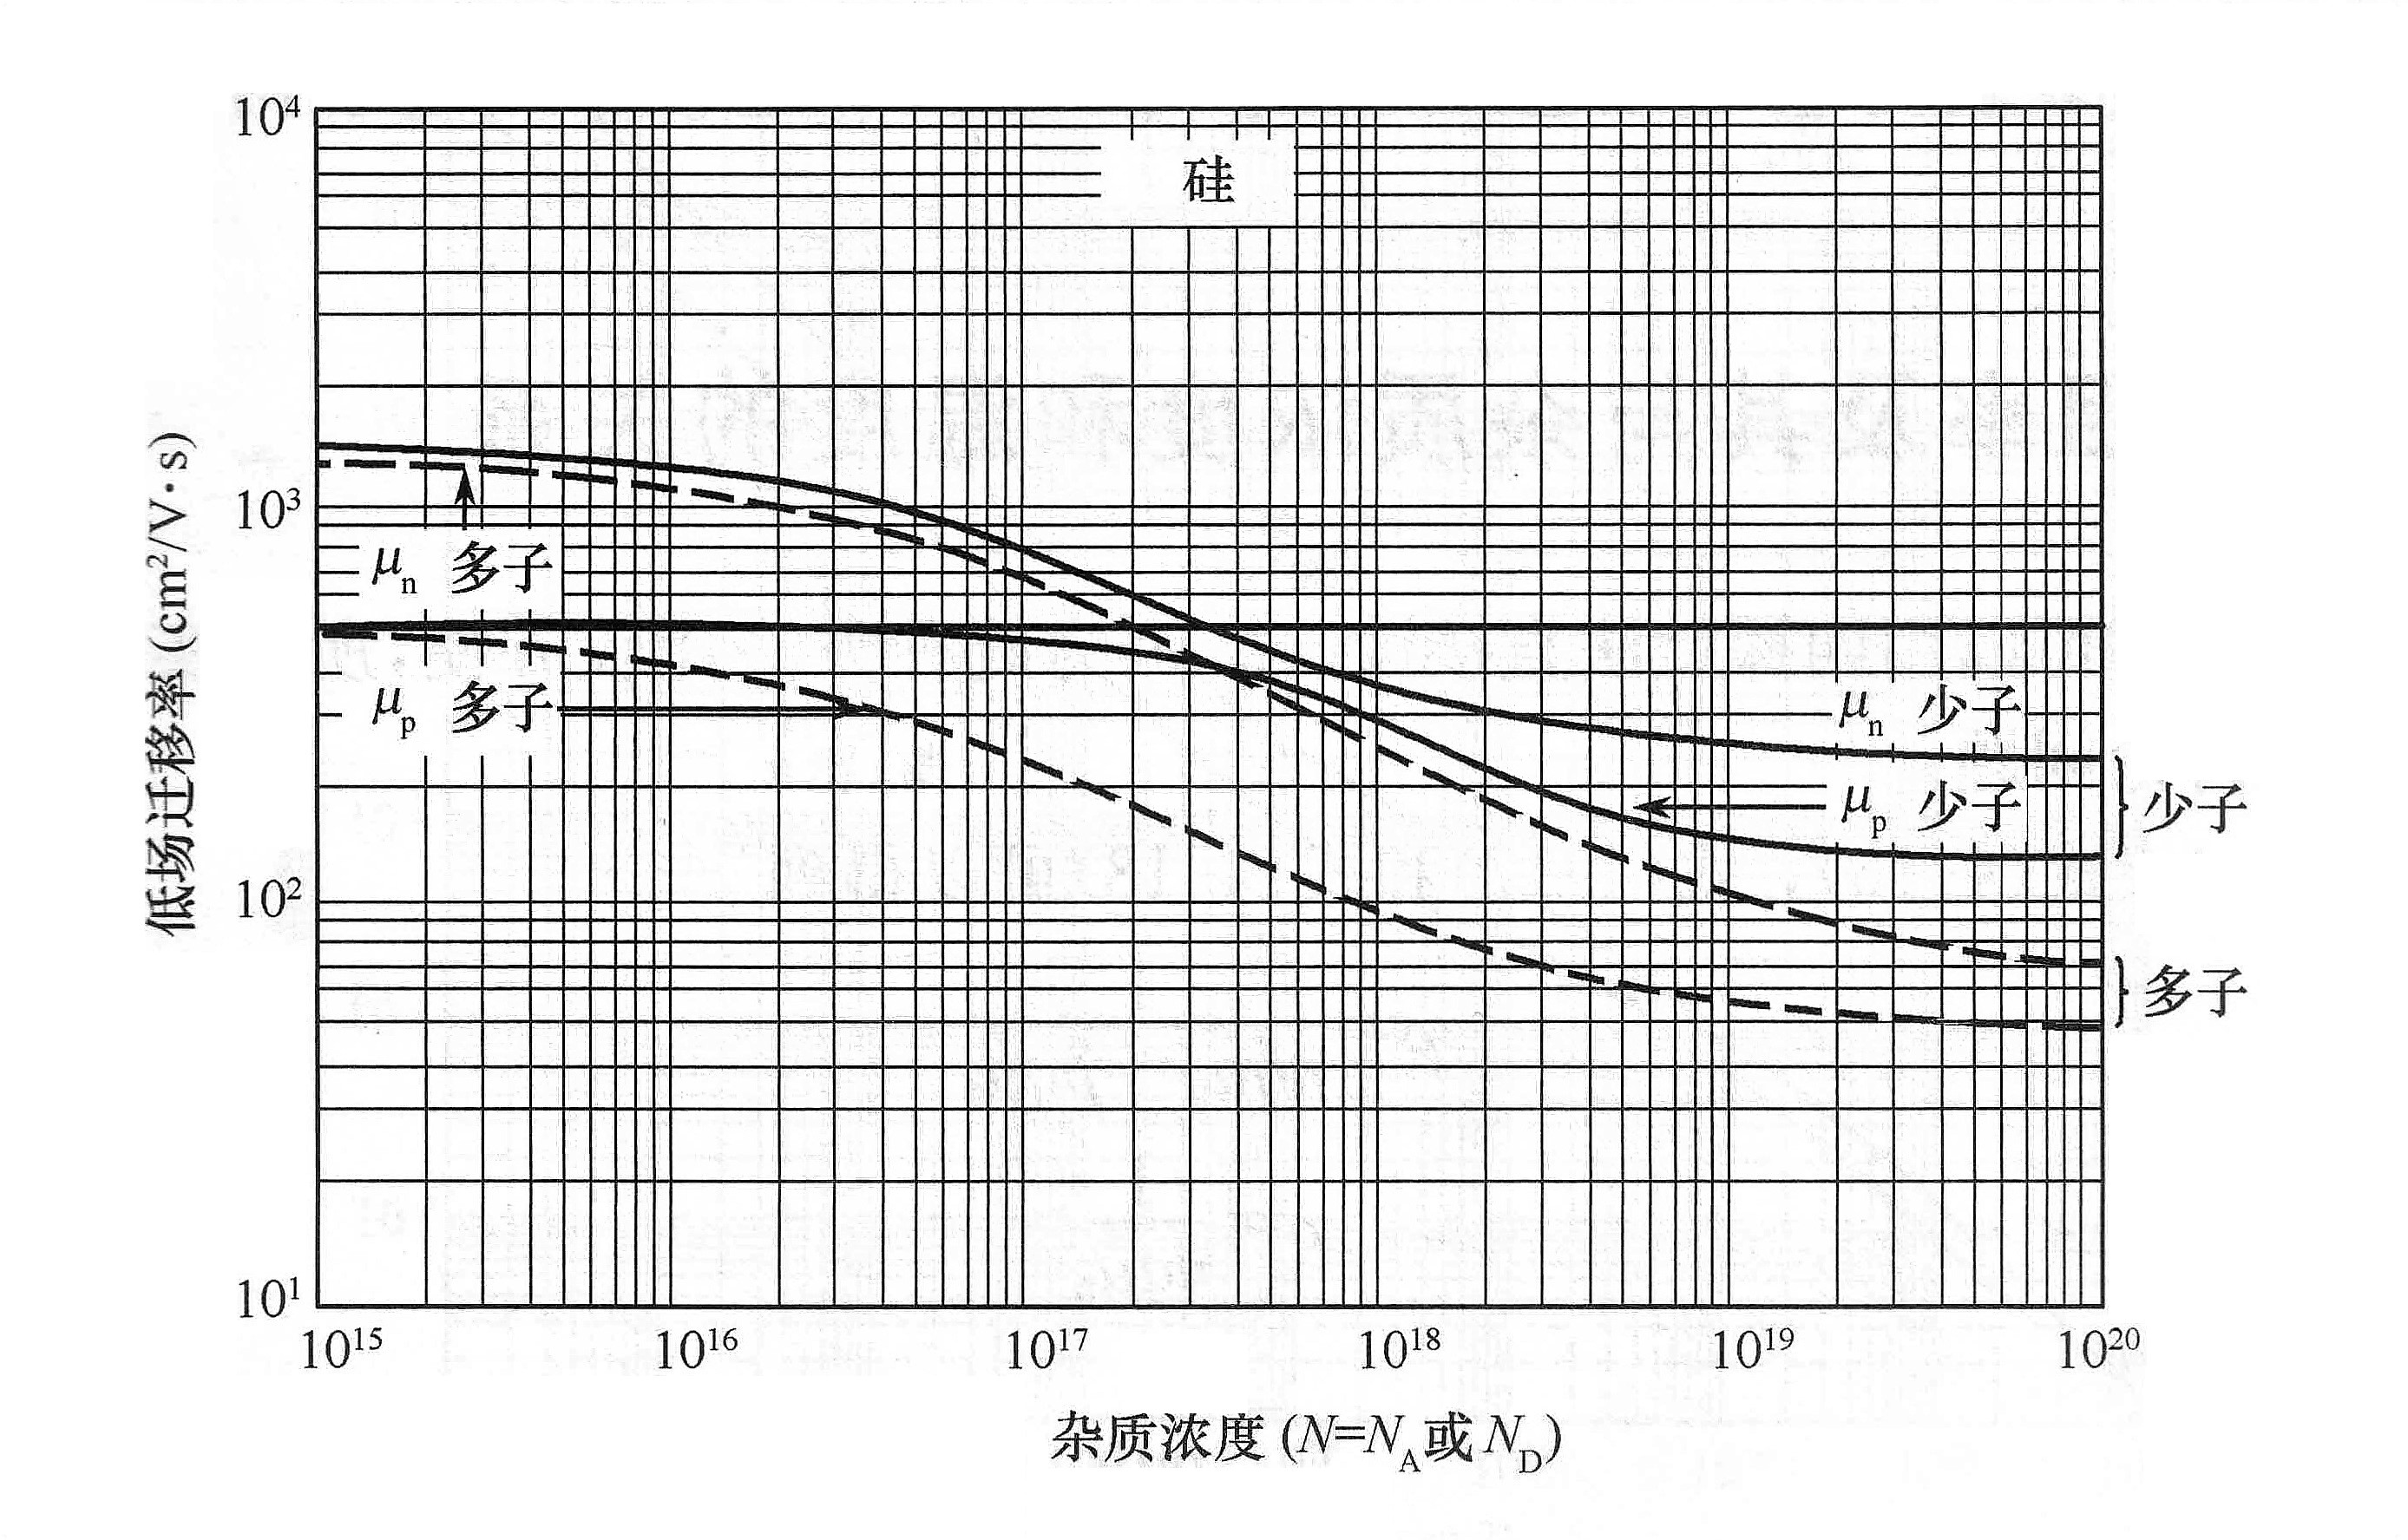
\includegraphics[width=12cm]{image/mu_N.jpg}
\end{Figure}


在\xref{tab:室温时较纯净半导体的迁移率}中,我们列出了室温下硅、锗、砷化镓在比较纯净时的迁移率数据。
\begin{Table}[室温时较纯净半导体的迁移率]
    <材料&电子迁移率$\mu_\text{n}$\quad\si{cm^2. V^{-1}. s^{-1}}&空穴迁移率$\mu_\text{p}$\quad\si{cm^2. V^{-1}. s^{-1}}\\>
    硅&1450&500\\
    锗&3800&1800\\
    砷化镓&8000&400\\
\end{Table}
还要指出的是,对于补偿材料,载流子浓度决定于两种杂质的浓度之差,但是,载流子迁移率则与两种杂质的浓度之和有关,例如对于$N_\text{D}>N_\text{A}$的情形,若全部电离,则
\begin{Equation}
    n=N_\text{D}-N_\text{A}\qquad
    N_\text{i}=N_\text{D}+N_\text{A}
\end{Equation}
由此可见,补偿的杂质半导体并不能等同于浓度相减,仅掺有单种杂质的杂质半导体。